\question (青岛大学,2001年)利用二叉链表存储树,则根结点的右指针是( )
\par\twoch{指向最左孩子}{指向最右孩子}{\textcolor{red}{空}}{非空}
\begin{solution}利用二叉链表存储树,需要先将树转换为二叉树,根据孩子兄弟表示法的规则,由于树的根结点一定没有右兄弟,所以转换为二叉树后,根结点一定是没有右孩子的。即根结点的右指针为空。本题选C。
\end{solution}
\question (北京航空航天大学,2002年)已知某完全二叉树采用顺序存储结构,结点数据信息的存放顺序依次为ABCDEFGH,该完全二叉树的后序遍历序列为(
)
\par\twoch{\textcolor{red}{HDEBFGCA}}{HEDBFGCA}{HDEBAFGC}{HDEFGBCA}
\begin{solution}画出该完全二叉树的示意图(下图)后,易得其后序遍历序列为HDEBFGCA,故本题选A。
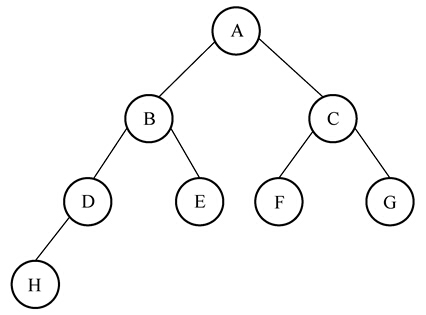
\includegraphics[width=2.08333in,height=2.08333in]{computerassets/82999f59b924ff27710fe8094367a64b.jpeg}
\end{solution}
\question (上海交通大学,2005年)在一棵具有n个节点的二叉树中,所有节点的空子树的个数等于(
)
\par\twoch{n}{n-1}{\textcolor{red}{n+1}}{2*n}
\begin{solution}一个简单的方法是将所有的空链域看成一棵子树,这样,原来所有的节点都是双分支节点,根据叶子节点数=双分支节点数+1,此时这里的叶子节点是原来的空链域,即n+1
\end{solution}
\question (中南大学,2005年)有n个节点的完全二叉树采用顺序存储结构,从根节点开始对其层次顺序进行编号(设根结点编号为1),下列说法错误的是(
)
\par\fourch{当1≤i≤n/2,节点i的左子女是节点2i,否则节点i没有左子女}{当1≤i≤(n-1)/2时,节点i的右子女是节点2i+1,否则节点i没有右子女}{\textcolor{red}{1≤i≤n时,节点i的父母节点是i/2(向下取整)}}{当i为偶数且1≤i≤n时,节点i的父母节点是i/2}
\begin{solution}对于C选项,如果i=1,则根节点的父母节点为0,而根节点没有父母节点,所以错误
\end{solution}
